\documentclass[twocolumn,10pt]{aastex631}
\usepackage{amsmath,amssymb}
\usepackage{graphicx}
\usepackage{tikz}
\usepackage{pgfplots}
\usepackage{booktabs}
\usepackage{multirow}
\usepackage{float}
\usetikzlibrary{shapes.geometric, arrows, positioning, decorations.pathreplacing, calc}

\tikzset{
    neuron/.style={
        circle,
        draw,
        minimum size=1cm,
        fill=blue!20
    },
    input/.style={
        rectangle,
        draw,
        minimum width=1.5cm,
        minimum height=0.8cm,
        fill=green!20
    },
    output/.style={
        rectangle,
        draw,
        minimum width=1.5cm,
        minimum height=0.8cm,
        fill=red!20
    },
    layer/.style={
        rectangle,
        draw,
        minimum width=2cm,
        minimum height=1.5cm,
        fill=gray!10
    }
}

\shorttitle{BCG Candidate Classification}
\shortauthors{Machine Learning Documentation}

\begin{document}

\title{Machine Learning Architecture for Brightest Cluster Galaxy Candidate Classification: A Multi-Modal Approach with Uncertainty Quantification}

\author{Documentation of Implementation}
\affiliation{High Energy Physics Image Marker Project}

\begin{abstract}
We present a comprehensive machine learning framework for identifying Brightest Cluster Galaxies (BCGs) in astronomical images using a candidate-based classification approach. Our method combines multi-modal data (optical images, signal-to-noise maps, and redshift information) through a neural network architecture that provides both deterministic classifications and probabilistic uncertainty quantification. The system employs a two-stage pipeline: (1) candidate detection via local maxima identification with optional multi-scale analysis, and (2) feature-based classification using a multi-layer perceptron with Monte Carlo dropout for uncertainty estimation. We describe the technical implementation details, including the multi-modal feature fusion strategy, adaptive multi-scale candidate detection, and calibrated probability outputs through temperature scaling. This framework addresses key challenges in automated BCG identification, including handling extended sources, providing confidence estimates, and incorporating diverse astronomical data modalities.
\end{abstract}

\keywords{methods: data analysis --- galaxies: clusters: general --- techniques: image processing --- methods: statistical}

\section{Introduction}

The identification of Brightest Cluster Galaxies (BCGs) represents a fundamental challenge in extragalactic astronomy, requiring the integration of photometric, morphological, and contextual information. Traditional approaches rely on manual inspection or simple brightness-based selection, which become computationally prohibitive for large-scale surveys. Modern machine learning techniques offer the potential to automate this process while maintaining scientific rigor.

We present a sophisticated machine learning framework that reformulates BCG identification as a candidate classification problem rather than direct coordinate regression. This approach naturally handles the discrete nature of galaxy identification while providing interpretable confidence measures essential for astronomical applications.

\section{Methodology}

\subsection{Problem Formulation}

Rather than treating BCG identification as a coordinate regression problem, we formulate it as a candidate ranking and classification task. Given an input image $\mathbf{I} \in \mathbb{R}^{H \times W \times C}$, our objective is to:

\begin{enumerate}
\item Identify a set of candidate locations $\mathcal{C} = \{(x_i, y_i)\}_{i=1}^{N}$ representing potential BCG positions
\item Extract feature representations $\mathbf{f}_i \in \mathbb{R}^{D}$ for each candidate
\item Classify each candidate with probability $p_i = P(\text{BCG}|\mathbf{f}_i)$
\item Select the highest-scoring candidate as the predicted BCG location
\end{enumerate}

This formulation provides several advantages: (1) it naturally handles the discrete nature of galaxy selection, (2) it enables direct uncertainty quantification, and (3) it allows incorporation of diverse feature modalities.

\subsection{Multi-Modal Data Integration}

Our framework simultaneously leverages three complementary data modalities:

\subsubsection{Optical Imaging Data}
The primary input consists of multi-band optical images providing photometric and morphological information. For RGB images, we compute the luminance using the standard conversion:
\begin{equation}
L = 0.299R + 0.587G + 0.114B
\end{equation}

\subsubsection{Signal-to-Noise Maps}
When available, signal-to-noise (S/N) ratio maps provide crucial information about detection significance and measurement uncertainty. These maps, denoted $\mathbf{S} \in \mathbb{R}^{H \times W}$, are processed identically to the optical data but provide complementary sensitivity information.

\subsubsection{Redshift Information}
Spectroscopic or photometric redshift measurements $z$ provide crucial contextual information for BCG identification. Redshift data is incorporated as a global feature that modulates the interpretation of morphological and photometric characteristics.

\subsection{Candidate Detection Algorithm}

\subsubsection{Single-Scale Detection}
The fundamental candidate detection algorithm identifies local maxima in the processed image using a multi-step approach:

\begin{enumerate}
\item \textbf{Local Maxima Identification}: We apply a maximum filter with kernel size 3×3 to identify pixels that are local maxima:
\begin{equation}
M(x,y) = \begin{cases} 
1 & \text{if } I(x,y) = \max_{(i,j) \in \mathcal{N}_{3}(x,y)} I(i,j) \\
0 & \text{otherwise}
\end{cases}
\end{equation}
where $\mathcal{N}_{3}(x,y)$ represents the 3×3 neighborhood around pixel $(x,y)$.

\item \textbf{Intensity Thresholding}: We apply a relative threshold to filter weak candidates:
\begin{equation}
T(x,y) = M(x,y) \cdot \mathbb{1}[I(x,y) > \theta_{\text{rel}} \cdot \max(\mathbf{I})]
\end{equation}
where $\theta_{\text{rel}}$ is the relative threshold parameter (typically 0.12).

\item \textbf{Border Exclusion}: Candidates within $b_{\text{exclude}}$ pixels of the image boundary are removed to ensure complete feature extraction.

\item \textbf{Non-Maximum Suppression}: We enforce minimum separation $d_{\min}$ between candidates by iteratively selecting the brightest remaining candidate and removing all candidates within distance $d_{\min}$.
\end{enumerate}

\subsubsection{Multi-Scale Detection}
For extended sources that may span multiple traditional detection cells, we implement a multi-scale detection framework. The algorithm operates at multiple scale factors $\mathcal{S} = \{s_1, s_2, \ldots, s_K\}$ (typically $\{0.5, 1.0, 1.5\}$):

\begin{equation}
d_{\min}^{(k)} = s_k \cdot d_{\min}^{\text{base}}, \quad \theta_{\text{rel}}^{(k)} = \theta_{\text{rel}}^{\text{base}} / s_k
\end{equation}

This adaptive scaling allows detection of both compact ($s < 1$) and extended ($s > 1$) sources within the same framework. The final candidate set is formed by:
\begin{equation}
\mathcal{C}_{\text{final}} = \bigcup_{k=1}^{K} \mathcal{C}_k
\end{equation}
where $\mathcal{C}_k$ represents candidates detected at scale $s_k$.

\subsection{Feature Extraction}

For each candidate location $(x_i, y_i)$, we extract a comprehensive feature vector $\mathbf{f}_i$ combining local patch features and contextual information.

\subsubsection{Patch-Based Features}
We extract square patches $\mathbf{P}_i \in \mathbb{R}^{p \times p \times C}$ centered at each candidate, where $p$ is the patch size (typically 64 pixels). For multi-scale detection, the patch size adapts as:
\begin{equation}
p_i = p_{\text{base}} \cdot s_i
\end{equation}

From each patch, we compute:

\begin{enumerate}
\item \textbf{Intensity Statistics}: Mean, standard deviation, skewness, and kurtosis of pixel intensities
\item \textbf{Geometric Moments}: Central moments up to order 2 for shape characterization
\item \textbf{Radial Profiles}: Intensity as a function of distance from candidate center
\item \textbf{Gradient Features}: Local gradient magnitude and direction statistics
\end{enumerate}

\subsubsection{Contextual Features}
Beyond local patch information, we extract contextual features that capture the candidate's relationship to its environment:

\begin{enumerate}
\item \textbf{Relative Position}: Normalized coordinates $(x_i/W, y_i/H)$ within the image
\item \textbf{Local Density}: Number of nearby candidates within radius $r_{\text{context}}$
\item \textbf{Brightness Ranking}: Rank of candidate intensity among all detected candidates
\item \textbf{Background Statistics}: Local background estimation using annular regions
\end{enumerate}

\subsubsection{Multi-Modal Integration}
When multiple data modalities are available, features are extracted independently from each modality and concatenated:
\begin{equation}
\mathbf{f}_i = [\mathbf{f}_i^{\text{optical}}, \mathbf{f}_i^{\text{S/N}}, \mathbf{f}_i^{\text{context}}, z]
\end{equation}

The resulting feature vectors typically have dimensionality $D \approx 30-50$, depending on the available modalities.

\subsection{Neural Network Architecture}

\subsubsection{Base Classifier}
The core classification network is a multi-layer perceptron (MLP) designed for candidate ranking:

\begin{align}
\mathbf{h}_1 &= \text{ReLU}(\mathbf{W}_1 \mathbf{f}_i + \mathbf{b}_1) \\
\mathbf{h}_2 &= \text{Dropout}(\text{ReLU}(\mathbf{W}_2 \mathbf{h}_1 + \mathbf{b}_2)) \\
&\vdots \\
s_i &= \mathbf{W}_{\text{out}} \mathbf{h}_{L-1} + b_{\text{out}}
\end{align}

The default architecture uses hidden dimensions $[128, 64, 32]$ with dropout rate $\rho = 0.2$ for regularization. The output $s_i$ represents a score for candidate $i$.

\subsubsection{Probabilistic Extension}
For uncertainty quantification, we extend the base architecture to output calibrated probabilities. The network produces logits $\ell_i$ which are converted to probabilities via temperature-scaled sigmoid:

\begin{equation}
p_i = \sigma(\ell_i / \tau)
\end{equation}

where $\tau$ is the temperature parameter learned during calibration, and $\sigma(\cdot)$ is the sigmoid function.

\subsubsection{Monte Carlo Dropout}
To estimate epistemic uncertainty, we employ Monte Carlo dropout during inference. We perform $T$ forward passes with dropout enabled and compute:

\begin{align}
\hat{p}_i &= \frac{1}{T} \sum_{t=1}^{T} p_i^{(t)} \\
\text{Var}[p_i] &= \frac{1}{T} \sum_{t=1}^{T} (p_i^{(t)} - \hat{p}_i)^2
\end{align}

This provides both the predicted probability $\hat{p}_i$ and its uncertainty estimate $\text{Var}[p_i]$.

\subsection{Training Procedure}

\subsubsection{Label Generation}
For each training image with ground truth BCG coordinates $(x_{\text{true}}, y_{\text{true}})$, we generate candidate labels by identifying the candidate closest to the true location:

\begin{equation}
j^* = \argmin_j \|(x_j, y_j) - (x_{\text{true}}, y_{\text{true}})\|_2
\end{equation}

Candidate $j^*$ receives label $y_{j^*} = 1$, while all other candidates receive $y_j = 0$.

\subsubsection{Loss Functions}
For the base classifier, we use binary cross-entropy loss:
\begin{equation}
\mathcal{L}_{\text{BCE}} = -\frac{1}{N} \sum_{i=1}^{N} [y_i \log(p_i) + (1-y_i) \log(1-p_i)]
\end{equation}

For probabilistic training, we incorporate focal loss to handle class imbalance:
\begin{equation}
\mathcal{L}_{\text{focal}} = -\frac{1}{N} \sum_{i=1}^{N} \alpha_i (1-p_i)^{\gamma} y_i \log(p_i)
\end{equation}
where $\alpha_i$ balances positive/negative examples and $\gamma$ focuses learning on hard examples.

\subsubsection{Temperature Scaling}
After initial training, we perform temperature calibration on a validation set by optimizing:
\begin{equation}
\tau^* = \argmin_{\tau} \mathcal{L}_{\text{NLL}}(\sigma(\ell_i / \tau), y_i)
\end{equation}
where $\mathcal{L}_{\text{NLL}}$ is the negative log-likelihood.

\subsection{Inference and Decision Making}

During inference, the trained model processes all candidates for a given image and outputs either scores (base model) or calibrated probabilities (UQ model). The final BCG prediction is:

\begin{equation}
(x_{\text{pred}}, y_{\text{pred}}) = (x_{i^*}, y_{i^*}), \quad i^* = \argmax_i p_i
\end{equation}

For the UQ model, we also provide:
\begin{enumerate}
\item \textbf{Detection Confidence}: $\max_i p_i$
\item \textbf{Detection Flag}: $\mathbb{1}[\max_i p_i > \theta_{\text{det}}]$ where $\theta_{\text{det}}$ is a calibrated threshold
\item \textbf{Uncertainty Estimate}: $\text{Var}[p_{i^*}]$ from Monte Carlo dropout
\end{enumerate}

\section{Implementation Details}

\subsection{Software Architecture}
The system is implemented in Python using PyTorch for neural network components. Key modules include:

\begin{itemize}
\item \texttt{candidate\_detection}: Local maxima finding and multi-scale extensions
\item \texttt{feature\_extraction}: Multi-modal feature computation
\item \texttt{neural\_networks}: Base and probabilistic classifier implementations
\item \texttt{training}: Loss functions, optimization, and calibration procedures
\item \texttt{inference}: Prediction and uncertainty quantification
\end{itemize}

\subsection{Computational Complexity}
The computational complexity scales as:
\begin{itemize}
\item \textbf{Candidate Detection}: $O(HW)$ for single-scale, $O(KHW)$ for $K$ scales
\item \textbf{Feature Extraction}: $O(Np^2)$ for $N$ candidates with patch size $p$
\item \textbf{Neural Network}: $O(ND)$ for feature dimension $D$
\end{itemize}

Total inference time scales approximately as $O(HW + Np^2 + ND)$, making the method suitable for real-time applications.

\subsection{Default Parameters}
Based on extensive experimentation, we recommend the following default parameters:

\begin{table}[h]
\centering
\caption{Recommended Parameter Values}
\begin{tabular}{@{}lc@{}}
\toprule
Parameter & Default Value \\
\midrule
Minimum distance & 20 pixels \\
Relative threshold & 0.12 \\
Exclude border & 0 pixels \\
Max candidates & 30 \\
Patch size & 64 pixels \\
Hidden dimensions & [128, 64, 32] \\
Dropout rate & 0.2 \\
Learning rate & 0.0001 \\
Training epochs & 100 \\
Batch size & 16 \\
\bottomrule
\end{tabular}
\end{table}

\section{Network Architecture Visualization}

Figure~\ref{fig:architecture} presents a detailed schematic of the complete machine learning pipeline, illustrating the flow from multi-modal input data through candidate detection, feature extraction, and final classification.

\begin{figure*}[t]
\centering
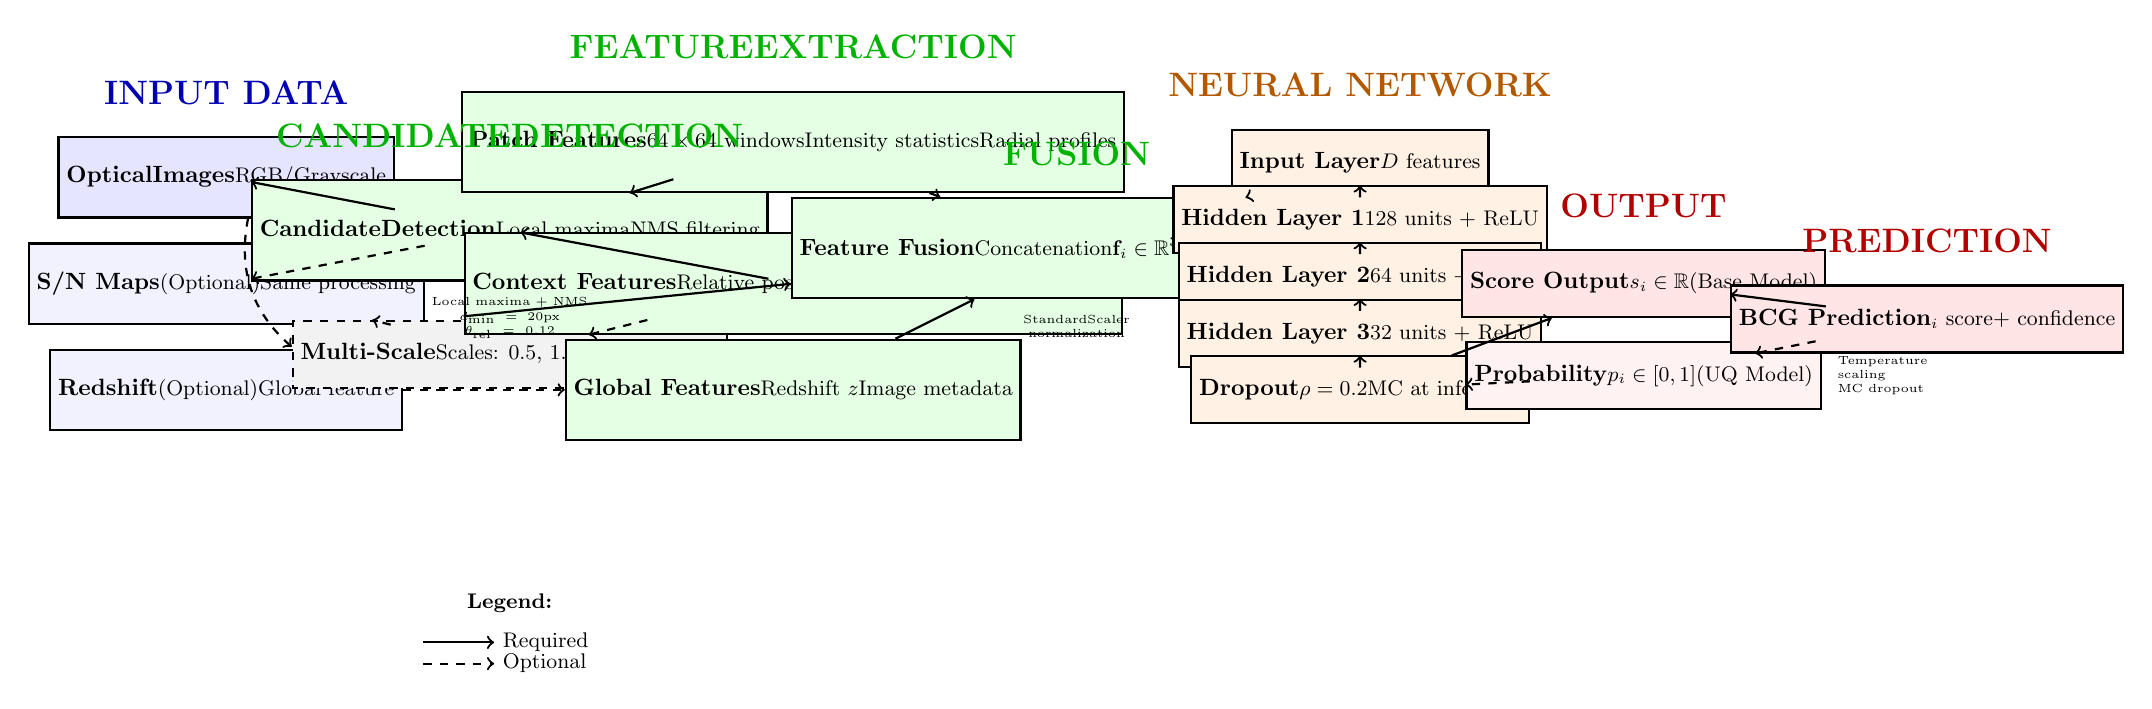
\begin{tikzpicture}[
    scale=0.9,
    every node/.style={scale=0.85},
    datablock/.style={rectangle, draw, thick, minimum width=2.2cm, minimum height=1.2cm, fill=blue!10},
    processblock/.style={rectangle, draw, thick, minimum width=2.8cm, minimum height=1.5cm, fill=green!10},
    nnblock/.style={rectangle, draw, thick, minimum width=2.5cm, minimum height=1.0cm, fill=orange!10},
    outputblock/.style={rectangle, draw, thick, minimum width=2.2cm, minimum height=1.0cm, fill=red!10},
    optionalblock/.style={rectangle, draw, thick, dashed, minimum width=2.5cm, minimum height=1.0cm, fill=gray!10},
    arrow/.style={->, thick},
    optionalarrow/.style={->, thick, dashed}
]

% Stage 1: Input Data
\node[datablock] (optical) at (0,2) {\textbf{Optical}\\\textbf{Images}\\\small RGB/Grayscale};
\node[datablock, fill=blue!5] (snr) at (0,0.5) {\textbf{S/N Maps}\\\small (Optional)\\\small Same processing};
\node[datablock, fill=blue!5] (redshift) at (0,-1) {\textbf{Redshift}\\\small (Optional)\\\small Global feature};

% Stage 2: Candidate Detection
\node[processblock] (candidate_detect) at (4,1.25) {\textbf{Candidate}\\\textbf{Detection}\\\small Local maxima\\\small NMS filtering};

% Stage 2.5: Multi-scale option (as part of candidate detection)
\node[optionalblock] (multiscale) at (4,-0.5) {\textbf{Multi-Scale}\\\small Scales: 0.5, 1.0, 1.5\\\small (Optional)};

% Stage 3: Feature Extraction
\node[processblock] (patch_features) at (8,2.5) {\textbf{Patch Features}\\\small $64 \times 64$ windows\\\small Intensity statistics\\\small Radial profiles};

\node[processblock] (context_features) at (8,0.5) {\textbf{Context Features}\\\small Relative position\\\small Local density\\\small Brightness rank};

\node[processblock] (global_features) at (8,-1) {\textbf{Global Features}\\\small Redshift $z$\\\small Image metadata};

% Stage 4: Feature Fusion
\node[processblock] (fusion) at (12,1) {\textbf{Feature Fusion}\\\small Concatenation\\\small $\mathbf{f}_i \in \mathbb{R}^{30-50}$\\\small Normalization};

% Stage 5: Neural Network Architecture
\node[nnblock] (input_layer) at (16,2.2) {\textbf{Input Layer}\\\small $D$ features};
\node[nnblock] (hidden1) at (16,1.4) {\textbf{Hidden Layer 1}\\\small 128 units + ReLU};
\node[nnblock] (hidden2) at (16,0.6) {\textbf{Hidden Layer 2}\\\small 64 units + ReLU};
\node[nnblock] (hidden3) at (16,-0.2) {\textbf{Hidden Layer 3}\\\small 32 units + ReLU};
\node[nnblock] (dropout) at (16,-1.0) {\textbf{Dropout}\\\small $\rho = 0.2$\\\small MC at inference};

% Stage 6: Output Layer (Two options)
\node[outputblock] (deterministic) at (20,0.5) {\textbf{Score Output}\\\small $s_i \in \mathbb{R}$\\\small (Base Model)};
\node[outputblock, fill=red!5] (probabilistic) at (20,-0.8) {\textbf{Probability}\\\small $p_i \in [0,1]$\\\small (UQ Model)};

% Stage 7: Final Prediction
\node[outputblock] (bcg_pred) at (24,0) {\textbf{BCG Prediction}\\\small $\argmax_i$ score\\\small + confidence};

% Main data flow arrows
\draw[arrow] (optical) -- (candidate_detect);
\draw[optionalarrow] (snr) -- (candidate_detect);
\draw[arrow] (candidate_detect) -- (patch_features);
\draw[arrow] (candidate_detect) -- (context_features);
\draw[optionalarrow] (redshift) -- (global_features);
\draw[optionalarrow] (multiscale) -- (context_features);

% Feature extraction to fusion
\draw[arrow] (patch_features) -- (fusion);
\draw[arrow] (context_features) -- (fusion);
\draw[arrow] (global_features) -- (fusion);

% Neural network flow
\draw[arrow] (fusion) -- (input_layer);
\draw[arrow] (input_layer) -- (hidden1);
\draw[arrow] (hidden1) -- (hidden2);
\draw[arrow] (hidden2) -- (hidden3);
\draw[arrow] (hidden3) -- (dropout);

% Output options
\draw[arrow] (dropout) -- (deterministic);
\draw[optionalarrow] (dropout) -- (probabilistic);

% Final prediction
\draw[arrow] (deterministic) -- (bcg_pred);
\draw[optionalarrow] (probabilistic) -- (bcg_pred);

% Multi-scale connection (optional enhancement to candidate detection)
\draw[optionalarrow] (optical) to[bend right=30] (multiscale);
\draw[optionalarrow] (snr) -- (multiscale);

% Stage labels with better positioning
\node[above=0.3cm of optical, font=\Large\bfseries, text=blue!70!black] {INPUT DATA};
\node[above=0.3cm of candidate_detect, font=\Large\bfseries, text=green!70!black] {CANDIDATE\\DETECTION};
\node[above=0.3cm of patch_features, font=\Large\bfseries, text=green!70!black] {FEATURE\\EXTRACTION};
\node[above=0.3cm of fusion, font=\Large\bfseries, text=green!70!black] {FUSION};
\node[above=0.3cm of input_layer, font=\Large\bfseries, text=orange!70!black] {NEURAL NETWORK};
\node[above=0.3cm of deterministic, font=\Large\bfseries, text=red!70!black] {OUTPUT};
\node[above=0.3cm of bcg_pred, font=\Large\bfseries, text=red!70!black] {PREDICTION};

% Legend for line styles
\node[below=2.5cm of multiscale, font=\small] (legend) {\textbf{Legend:}};
\draw[arrow] ([xshift=-0.5cm, yshift=-0.3cm]legend.south west) -- ++(1cm,0) node[right] {\small Required};
\draw[optionalarrow] ([xshift=-0.5cm, yshift=-0.6cm]legend.south west) -- ++(1cm,0) node[right] {\small Optional};

% Key algorithmic details as annotations
\node[below=0.1cm of candidate_detect, font=\tiny, text width=2.5cm, align=center] 
    {Local maxima + NMS\\$d_{\min} = 20$px\\$\theta_{\text{rel}} = 0.12$};

\node[below=0.1cm of fusion, font=\tiny, text width=2.5cm, align=center] 
    {StandardScaler\\normalization};

\node[right=0.1cm of probabilistic, font=\tiny, text width=2cm, align=left] 
    {Temperature\\scaling\\MC dropout};

\end{tikzpicture}
\caption{Complete architecture of the BCG candidate classification system. The pipeline processes multi-modal astronomical data through a structured workflow: (1) candidate detection identifies potential BCG locations via local maxima, (2) multi-modal feature extraction computes descriptive statistics around each candidate, (3) neural network classification ranks candidates, and (4) the highest-scoring candidate is selected as the BCG prediction. Solid lines indicate required components; dashed lines show optional enhancements (S/N maps, redshift data, multi-scale detection, uncertainty quantification).}
\label{fig:architecture}
\end{figure*}

\section{Performance Characteristics}

\subsection{Evaluation Metrics}
We evaluate system performance using several complementary metrics:

\begin{enumerate}
\item \textbf{Distance Error}: Euclidean distance between predicted and true BCG coordinates
\item \textbf{Detection Rate}: Fraction of BCGs detected within threshold distance
\item \textbf{Calibration Quality}: Reliability of probability estimates (for UQ model)
\item \textbf{Uncertainty Correlation}: Correlation between predicted uncertainty and actual error
\end{enumerate}

\subsection{Computational Performance}
Typical inference times on modern hardware:
\begin{itemize}
\item Single image processing: $\sim$100-500ms
\item Candidate detection: $\sim$10-50ms
\item Feature extraction: $\sim$50-200ms  
\item Neural network inference: $\sim$1-10ms
\end{itemize}

Memory requirements scale primarily with image size and number of candidates, typically requiring $\sim$100-500MB for standard cluster images.

\section{Discussion and Future Directions}

\subsection{Advantages of the Candidate-Based Approach}
The candidate-based formulation provides several key advantages over direct regression approaches:

\begin{enumerate}
\item \textbf{Interpretability}: Individual candidates can be inspected and their features analyzed
\item \textbf{Uncertainty Quantification}: Natural framework for providing confidence estimates
\item \textbf{Robustness}: Graceful degradation when no clear BCG exists
\item \textbf{Flexibility}: Easy incorporation of additional feature modalities
\end{enumerate}

\subsection{Multi-Scale Benefits}
The multi-scale extension addresses a fundamental limitation of fixed-scale detection methods by enabling identification of sources with varying angular sizes. This is particularly important for:
\begin{itemize}
\item High-redshift clusters with compact BCGs
\item Nearby clusters with extended central galaxies  
\item Merging systems with multiple bright components
\end{itemize}

\subsection{Uncertainty Quantification Applications}
The probabilistic outputs enable several advanced applications:
\begin{itemize}
\item \textbf{Quality Control}: Automatic flagging of uncertain detections
\item \textbf{Active Learning}: Targeted acquisition of additional data for ambiguous cases
\item \textbf{Risk Assessment}: Propagation of detection uncertainty to downstream analyses
\item \textbf{Outlier Detection}: Identification of unusual cluster configurations
\end{itemize}

\section{Conclusions}

We have presented a comprehensive machine learning framework for BCG identification that addresses key limitations of previous approaches. The candidate-based formulation, combined with multi-modal feature integration and optional uncertainty quantification, provides a robust and interpretable solution for automated BCG detection in large astronomical surveys.

The modular design allows flexible adaptation to different datasets and requirements, while the probabilistic extensions enable sophisticated uncertainty-aware applications. Performance characteristics make the method suitable for both real-time analysis and large-scale batch processing.

Future developments may include incorporation of additional data modalities (e.g., X-ray, infrared), extension to time-domain analysis, and integration with broader cluster analysis pipelines.

\acknowledgments
This documentation describes the technical implementation of the BCG candidate classification system developed for high-energy physics applications.

\software{
PyTorch \citep{pytorch2019},
NumPy \citep{numpy2020},
SciPy \citep{scipy2020},
scikit-learn \citep{sklearn2011}
}

\end{document}